% Paper 5 --- the evidentiary basis of a digital legal corpus.
% Footnote citations, venue-neutral until one is chosen. Compiles on a plain
% TeX Live; build.py produces the submission files.
\documentclass[11pt]{article}
\usepackage[a4paper,top=2.5cm,bottom=2.5cm,left=3cm,right=3cm]{geometry}
\usepackage{times}
\usepackage{setspace}
\onehalfspacing
\usepackage[hidelinks]{hyperref}

% Set \anontrue before producing the file uploaded to a journal that reviews
% anonymously.
\newif\ifanon
\anonfalse

\usepackage[T1]{fontenc}
\usepackage[utf8]{inputenc}
\usepackage{microtype}
\usepackage{booktabs}
\usepackage{graphicx}
\usepackage{url}
\emergencystretch=3em

\title{What It Took to Read the Law:\\
Access, Provenance and the Evidentiary Basis of a Digital Legal Corpus}

\ifanon
  \author{}
  \date{}
\else
  \author{Abdullah Almohammedi \\
    Independent Researcher \\
    \texttt{abdullah.m.almohammedi@gmail.com} \\
    ORCID: \href{https://orcid.org/0009-0001-0832-0995}{0009-0001-0832-0995}}
  \date{}
\fi

\begin{document}

\maketitle

\begin{abstract}
\noindent
Empirical legal research, legal information systems and legal AI all rest on
an assumption none of them states: that the official text of the law was
available, and was itself consistent, at the moment the text was collected.
This article tests that assumption against the record kept while building a
corpus of Saudi Arabian legislation. Every verified article carries a
provenance string naming the sources consulted and how they were reconciled,
and every instrument carries a hand-assigned verification tier. Measured over
the 11,704 articles whose record names its sources, the official source was
unreachable for 20.0 per cent of them, covering 28.0 per cent of instruments;
20.9 per cent were obtained through a web archive; 10.2 per cent rest on a
single source; 8.2 per cent required optical or visual reconstruction; and 4.9
per cent record a defect in the official text itself. Weighted by article, 17.0
per cent of the corpus has no cross-verified official primary source behind it,
and the coverage of the sample makes that an underestimate rather than an
overestimate. In four instruments the official record contradicts itself across nine
articles: the article the portal displays and the change log the same portal
publishes do not agree. Two conclusions follow. Web archives are not a convenience for legal
research but part of its load-bearing structure, with no guarantee of
permanence and no legal status. And a legal corpus should ship the strength of
the evidence behind each text alongside the text, because a reader who is given
only the text cannot tell the difference between a provision confirmed against
two official sources and one transcribed from a single scan.
\end{abstract}

\vspace{1em}\noindent\textbf{Keywords:} legal information; provenance; web
archiving; official sources; legal corpora; Saudi Arabia
\vspace{1.5em}

\section{Introduction}

Article 1 of the Saudi Environmental Law can be read on the official
legislative portal. It can also be read, on the same portal, in a form that
does not match. The corpus described below records the discrepancy against
that article, resolved only by going to two independent sources outside the
portal and taking the reading on which they agreed.\footnote{Environmental Law
(Royal Decree M/165, 19/11/1441H) art 1; the provenance record for the article
is published with the analysis code.}

That is an uncomfortable observation to build on, and it is not the point of
this article. The point is what it takes to notice. A researcher who consults
the portal once, on a good day, gets an answer and no reason to doubt it. The
discrepancy is visible only to someone who consulted the portal repeatedly, kept
a record of what each attempt returned, and compared. Almost nobody does that,
because almost nobody has reason to: the official source is where the law is,
and if the official source says something, that is what the law says.

This article examines what happens to that assumption when it is checked. It
uses a corpus of Saudi Arabian legislation in which every verified article
carries a provenance string naming the sources consulted and how they were
reconciled, together with a verification tier assigned by hand to each
instrument.\footnote{The corpus and the scripts that reproduce every number and
figure here are openly archived; see the data availability statement.} The
corpus was not built to study its own provenance. The record exists because
building it required deciding, article by article, whether the text in hand
could be relied on --- and the record of those decisions turns out to be
evidence about something larger than one corpus.

Three findings follow, and a fourth observation about this corpus's own
shortcomings.

First, \textbf{the official source was frequently not available}. For 20.0 per
cent of articles, covering 28.0 per cent of instruments, the build record
documents that the primary official source could not be reached: a portal
returning an error, a connection reset, a page that no longer resolved. This
is not a claim that the sources are badly maintained. It is a measurement of
how often a researcher who needs the official text will not get it on the
first attempt --- or the fifth.

Second, \textbf{web archives did much of the work instead}. 20.9 per cent of
articles were obtained through an archived capture rather than a live official
page. The two totals are close, but that alone would prove nothing --- so the
joint is measured rather than inferred: 67.8 per cent of the articles whose
official source was unreachable were recovered through an archive, and 65.1 per
cent of archive use coincided with a recorded unavailability. The archive
standing in for a page that would not load is therefore the dominant pattern
and not the only one; 7.3 per cent of articles used an archive with no
unavailability recorded, and 6.4 per cent record unavailability that an archive
did not resolve. The Internet Archive is not a fallback for this kind of
research. It is part of the infrastructure, and it holds that position without
any legal status, any guarantee of permanence, and no obligation to anyone.

Third, \textbf{the evidence behind the text is uneven, and nothing published
alongside the text says so}. Weighted by article, 64.2 per cent of the corpus
rests on two or more official sources in agreement; 18.9 per cent on one
official source cross-checked against secondary ones; 4.5 per cent on secondary
sources only, because no official source could be reached; and 12.5 per cent on
a single source or on evidence that varies within the instrument. A reader
given the consolidated text alone cannot distinguish the first case from the
last.

The fourth observation is about the record itself, and it cuts against the
corpus this article uses. The provenance field is free text, not a controlled
vocabulary, and 3,704 of 15,408 articles carry a value in it that is not a
provenance statement at all --- a lifecycle status such as `unchanged' that
leaked into the same field. A project that took provenance unusually seriously
still ended up with a provenance field that means three different things. That
is reported here rather than quietly cleaned, because it is the strongest
available argument that provenance needs a vocabulary and a schema rather than
a place to write a sentence.

\section{The assumption, and who relies on it}

\subsection{In citation practice}

Legal citation is built on the premise that a citation is a retrieval
instruction: it names an instrument and a provision so that a reader can go and
read it. The convention is old enough to predate the question of whether the
naming is enough, and it does not encode where the reader should go, or what
they should do if what they find there is not what the citing author found.

For most of the history of legal citation this was adequate, because the
authoritative artefact was a printed gazette held in libraries, and the
question `is this the text?' had a physical answer. It is less adequate when
the authoritative artefact is a database behind a web front end, whose contents
can change without notice and whose availability is a function of
infrastructure nobody involved in the citation controls.

\subsection{In empirical legal research and legal AI}

The exposure is sharper for work that consumes law at scale. A study measuring
the structure of a legal system, or a model trained or grounded on statutory
text, takes a snapshot and treats it as the law. Machine-readable legal corpora
have grown substantially in recent years, and their documentation concentrates
on size, licensing and composition rather than on how the text was obtained or
how strongly it is attested.\footnote{Peter Henderson and others, `Pile of Law:
Learning Responsible Data Filtering from the Law and a 256GB Open-Source Legal
Dataset' (NeurIPS 2022, Datasets and Benchmarks Track); Joel Niklaus and
others, `MultiLegalPile: A 689GB Multilingual Legal Corpus' (Proceedings of the
62nd Annual Meeting of the Association for Computational Linguistics, 2024).}
The dataset-documentation literature has argued for exactly this kind of
disclosure in general terms, and legal corpora have largely not adopted
it.\footnote{Timnit Gebru and others, `Datasheets for Datasets' (2021) 64
Communications of the ACM 86; Emily M Bender and Batya Friedman, `Data
Statements for Natural Language Processing' (2018) 6 Transactions of the
Association for Computational Linguistics 587.}

Structural standards for legislative documents can carry provenance metadata,
and the capacity has been available for years.\footnote{Monica Palmirani and
Fabio Vitali, `Akoma-Ntoso for Legal Documents' in \emph{Legislative XML for
the Semantic Web} (Springer 2011) 75.} The gap is not representational. It is
that nobody is required to fill the fields, and a corpus that leaves them empty
looks exactly like a corpus whose text is impeccable.

\subsection{In the archiving literature}

That legal citations rot is not a new observation. Zittrain, Albert and Lessig
found that more than 70 per cent of URLs cited in the \emph{Harvard Law Review}
and comparable journals, and 50 per cent of those in United States Supreme
Court opinions, no longer led to the material originally cited --- the finding
that produced Perma.cc.\footnote{Jonathan Zittrain, Kendra Albert and Lawrence
Lessig, `Perma: Scoping and Addressing the Problem of Link and Reference Rot in
Legal Citations' (2014) 127 Harvard Law Review Forum 176.} What that literature
measures is the failure of a citation to resolve some time after publication. This article measures
something adjacent and, for a corpus builder, more immediate: the failure of an
official source to resolve \emph{at the moment of collection}, when the
researcher is actively trying and has every incentive to succeed.

\section{Data and method}
\label{sec:method}

\subsection{The provenance record}

Each verified article in the corpus carries a status string written during the
build, naming the sources consulted and how they were reconciled --- for
example, that the Ministry of Justice portal's API text was cross-checked
against the official PDF from the same portal, or that the live official portal
was unreachable and the text rests on two independent secondary sources agreeing
word for word. There are 15,408 such articles and 158 distinct strings.

Each instrument also carries a verification tier assigned by hand: two or more
official sources in agreement (tier 1); one official source cross-checked
against secondary sources (tier 2); no official source reachable, secondary
sources only (tier 3); or a single source, or evidence that varies within the
instrument (tier 4).

\subsection{Classifying free text, and publishing the classification}

The status strings are not a controlled vocabulary, and treating them as one
would be the first mistake available. The analysis therefore classifies each
distinct string by an explicit rule and publishes the entire mapping, so that a
reader can disagree with any single assignment rather than having to accept the
totals.

A string counts as a \emph{provenance statement} when it names a source, an
artefact or a retrieval route --- a portal, a gazette, a named secondary site, a
PDF, an archive capture, an OCR pass. Strings that name none of these are not
provenance statements: they are lifecycle values such as `unchanged' or
`amended', and in one case a single Arabic word, that were written into the
same field. There are 3,704 such articles, 24.0 per cent of those carrying any
status at all. They are excluded from every measure below.

Within the provenance statements, six measures are computed by token match,
each reported as a share of articles and as a share of instruments. The
measures overlap by design: an instrument reached through an archive because
the live portal was down scores on both. Every count is published with its
underlying string table.

\subsection{Two decisions that changed the numbers}

Two methodological choices are recorded because each moved a headline, and a
reader is entitled to know which way.

\textbf{Weighting.} Measures are computed per article, not per instrument. A
single-source instrument of five articles and one of three hundred are not the
same exposure, and an instrument count cannot tell them apart. The two
denominators diverge in ways that are themselves informative: optical
reconstruction touches 8.2 per cent of articles but 14.0 per cent of
instruments, which is what it looks like when the hardest sources to obtain are
also the shortest documents.

\textbf{A prior estimate was wrong.} An earlier pass over the registry's
free-text notes, matching patterns against prose rather than against the
structured provenance field, suggested that 47 per cent of instruments recorded
an unreachable official source. The disciplined measure is 28.0 per cent of
instruments and 20.0 per cent of articles. The first figure was an artefact of
matching loosely-worded notes, and it is reported here because a reader
encountering both should know which to use and why.

\section{What it took to obtain the text}

\begin{figure}[t]
\centering
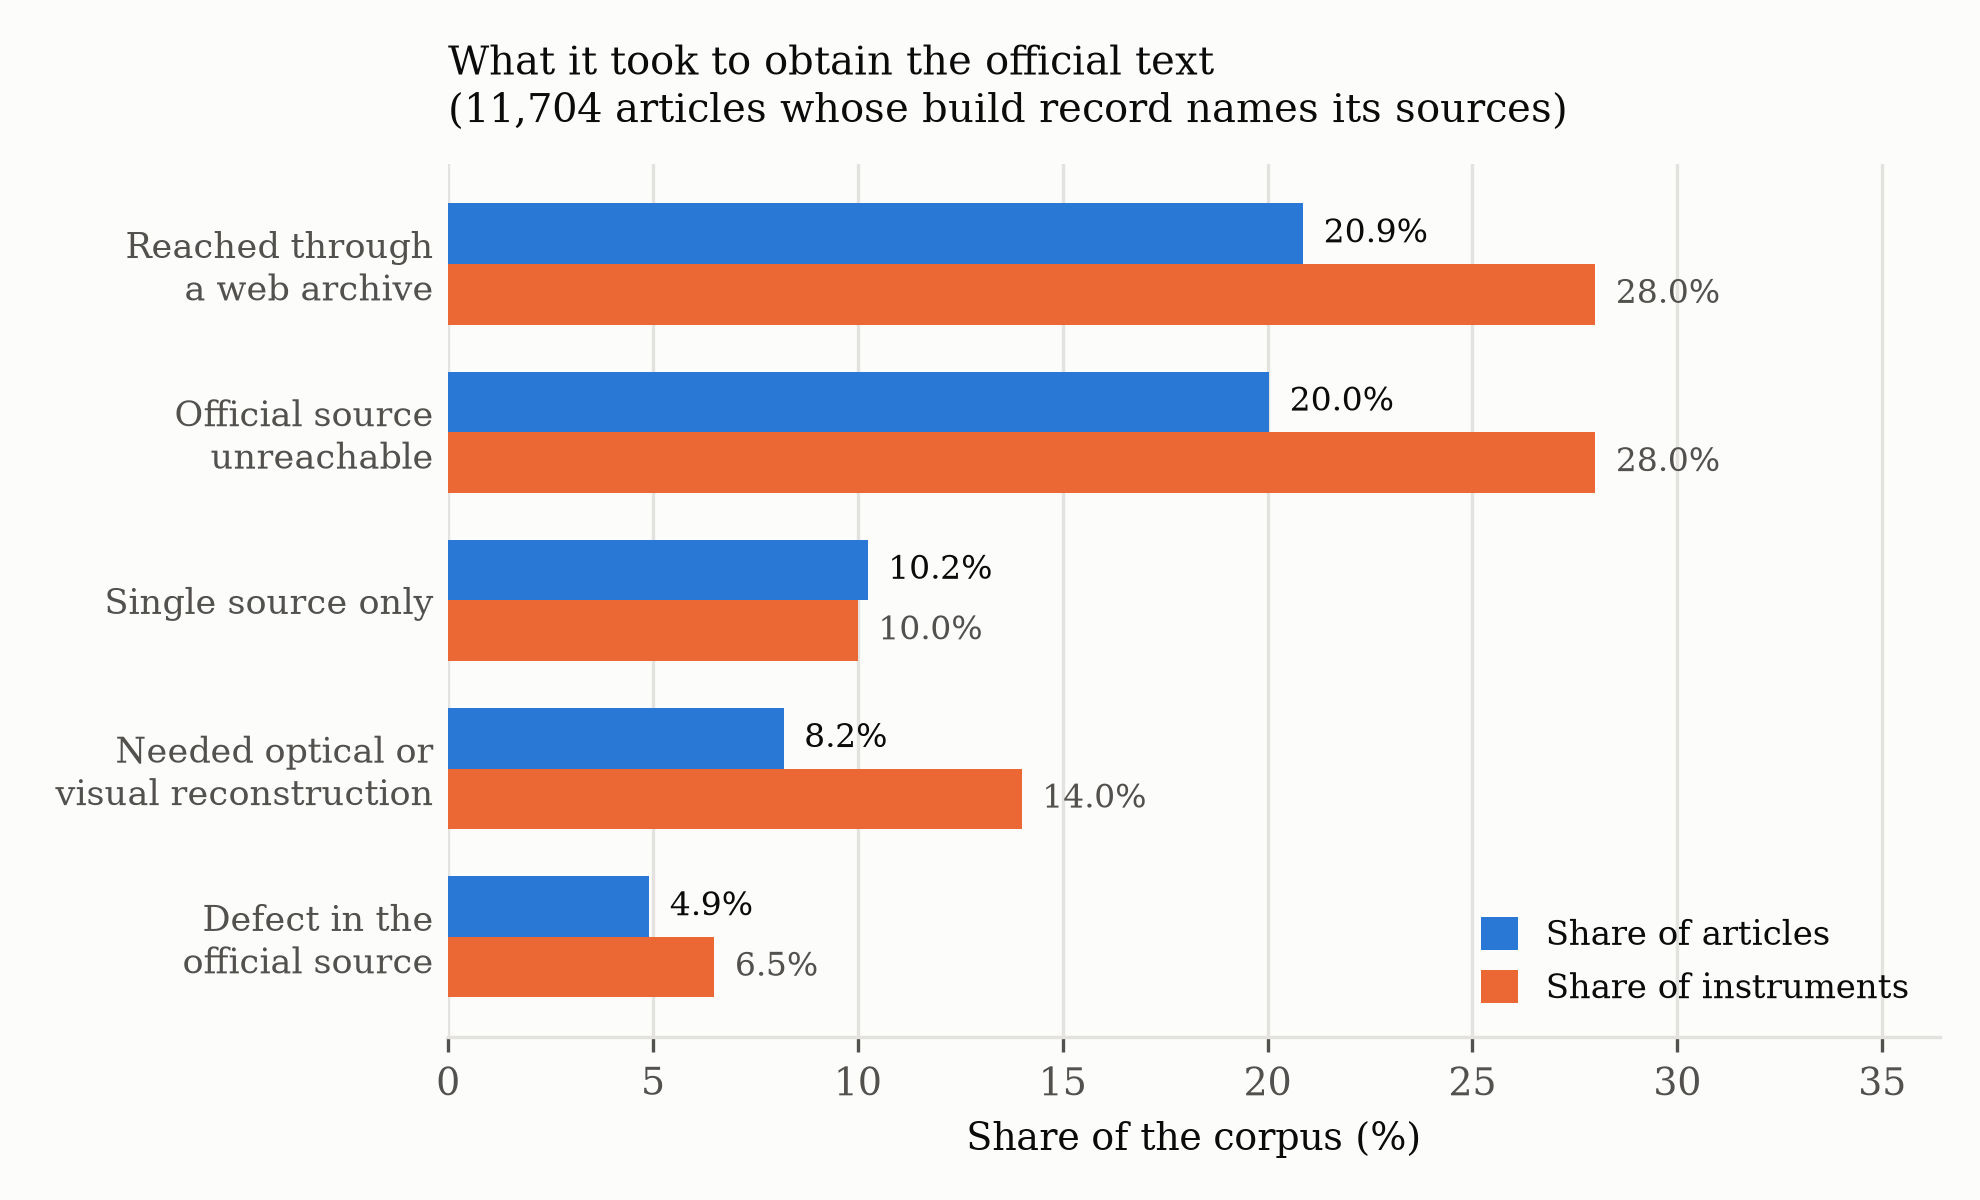
\includegraphics[width=\textwidth]{fig1_access.png}
\caption{The friction documented in the build record, as a share of articles
and of instruments. The measures overlap: an instrument reached through an
archive because the live portal was down appears in both of the top two rows.}
\label{fig:access}
\end{figure}

\begin{table}[t]
\centering
\small
\begin{tabular}{lrr}
\toprule
\textbf{} & \textbf{Articles} & \textbf{Instruments} \\
\midrule
Official source unreachable & 20.0\% & 28.0\% \\
Reached through a web archive & 20.9\% & 28.0\% \\
Single source only & 10.2\% & 10.0\% \\
Required optical or visual reconstruction & 8.2\% & 14.0\% \\
Defect recorded in the official source & 4.9\% & 6.5\% \\
\midrule
Multi-source cross-verification & 86.1\% & 87.5\% \\
\bottomrule
\end{tabular}
\caption{Measured over the 11,704 articles whose status field is a provenance
statement, across 200 instruments.}
\label{tab:access}
\end{table}

Table~\ref{tab:access} and Figure~\ref{fig:access} give the result. Four things
in it are worth drawing out.

\textbf{The last row is the good news and it should be read first.} 86.1 per
cent of articles were cross-verified against more than one source. This is not
a portrait of a corpus assembled carelessly from whatever was to hand, and the
other rows should be read in that light: they describe what a careful process
had to do, not what a careless one got away with.

\textbf{Unavailability and archive use are close, and they overlap by about
two thirds.} The totals are 20.0 per cent against 20.9 per cent, with 28.0 per
cent of instruments on both --- but matching totals do not establish that the
same articles are involved, so the joint distribution is computed. Of the
articles whose official source was unreachable, 67.8 per cent were recovered
through an archive; of the articles obtained through an archive, 65.1 per cent
had a recorded unavailability. The archive is mostly not supplying different or
better material: it is supplying the official material, at a moment when the
official channel could not. The remainders matter too, and neither is small:
852 articles used an archive with no unavailability recorded --- an archived
capture preferred for its stability, or consulted to check whether a live page
had changed --- and 754 record an unavailability that no archive resolved.

\textbf{Optical reconstruction is an instrument-level burden.} 8.2 per cent of
articles but 14.0 per cent of instruments. The sources that had to be read as
images --- scanned resolutions, PDFs with broken text layers, ministry
documents published as pictures of pages --- are disproportionately short
instruments. One in seven instruments in this corpus could not be read by
machine at all without an optical pass, and each such pass is an opportunity
for a silent error that no downstream user can detect.

\textbf{Defects in the official text are rarer than access failures but not
rare.} 4.9 per cent of articles carry a record of a defect in the source
itself: a typographical error preserved rather than silently corrected,
ligature corruption from PDF extraction, a scrambled text layer, a truncated
page. These are recorded because the build policy was to preserve source
defects verbatim and document them, rather than to tidy them. A corpus that
tidies them looks cleaner and tells its users less.

\section{The strength of the evidence}

\begin{figure}[t]
\centering
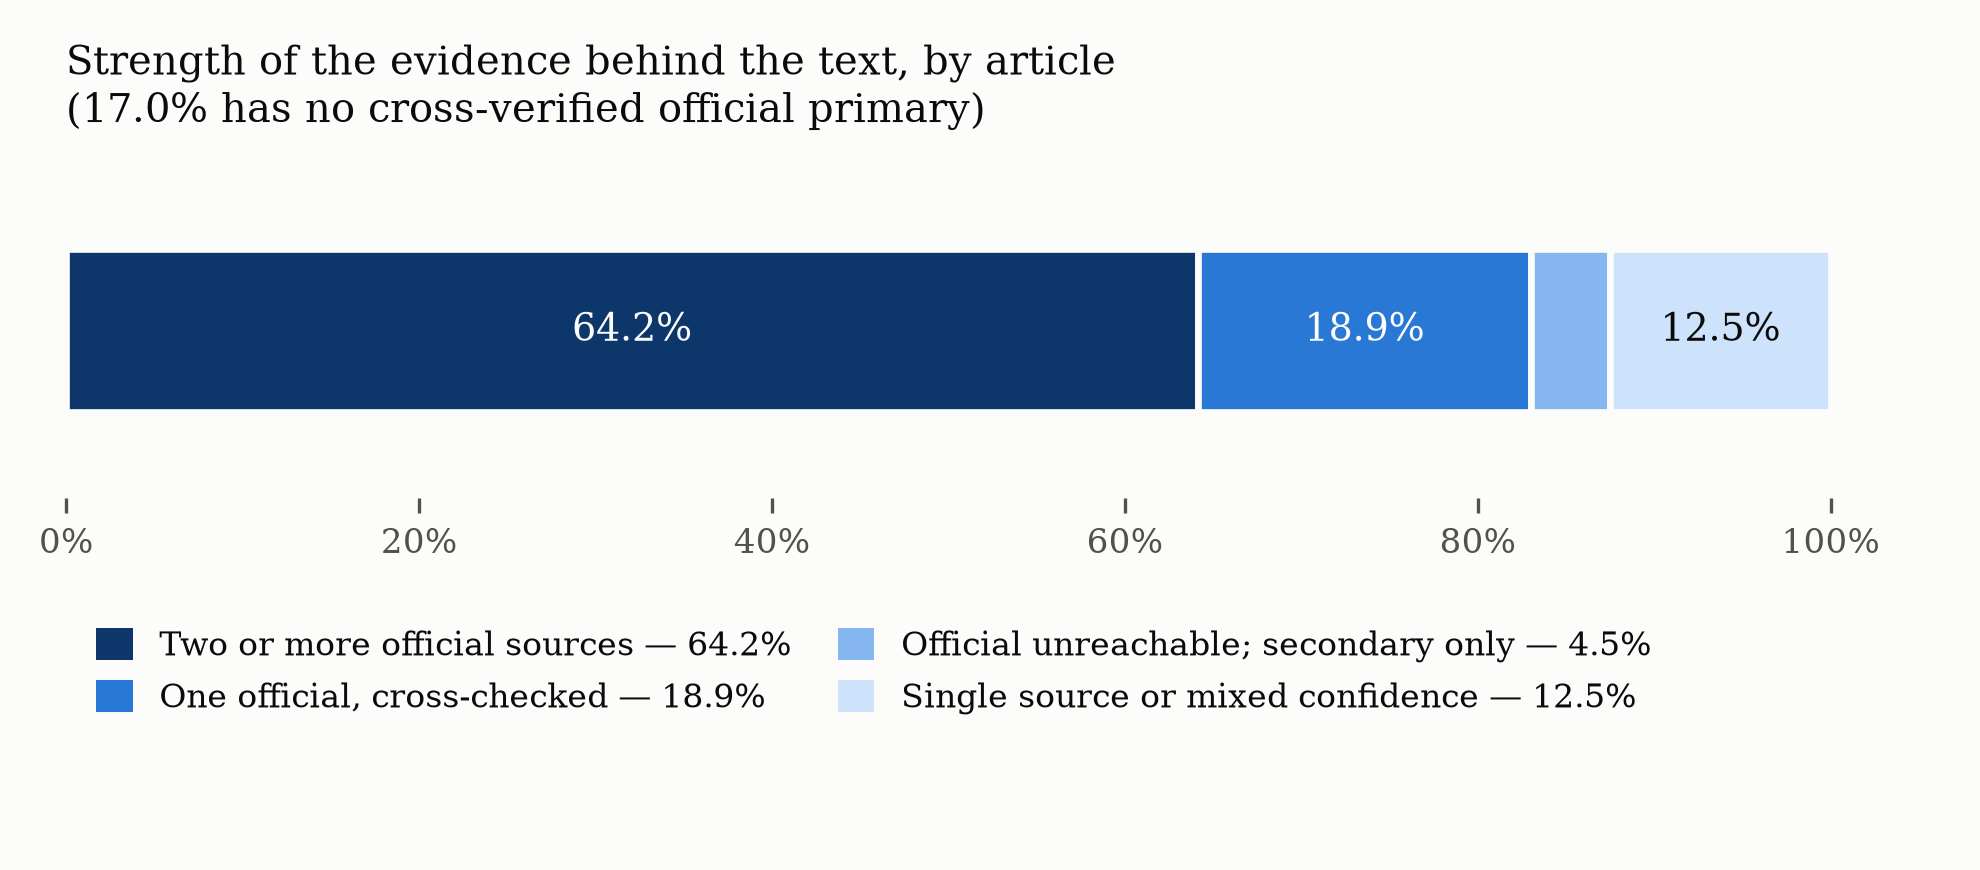
\includegraphics[width=\textwidth]{fig2_tiers.png}
\caption{Verification tiers weighted by article. The tiers are ordinal, from
two or more agreeing official sources to a single source or evidence that
varies within the instrument.}
\label{fig:tiers}
\end{figure}

Figure~\ref{fig:tiers} weights the hand-assigned tiers by article. Just under
two thirds of the corpus rests on two or more official sources in agreement.
The remaining third does not, and 17.0 per cent has no cross-verified official
primary source at all: 4.5 per cent because no official source could be reached,
and 12.5 per cent because the evidence is single-source or varies within the
instrument.

\subsection{The direction of the error}

That 17.0 per cent is an underestimate, and it is worth being precise about
why, because the alternative --- asserting that a convenient figure is
conservative --- is exactly the move a reader should distrust.

Not every instrument in the corpus has article-level verified records, and the
ones that do are not a random draw. Coverage by tier is 87 per cent for tier 1,
59 per cent for tier 2, 28 per cent for tier 3 and 73 per cent for tier 4. The
pattern is not monotonic, but tier 3 --- the instruments whose official source
could not be reached at all --- is by a wide margin the least represented. The
instruments most likely to be missing from the article-weighted measure are the
instruments whose evidence is weakest. A registry-wide count of instruments,
which does not have this problem, puts tiers 3 and 4 together at 76 of 291
instruments, or 26 per cent.

\section{When the official record disagrees with itself}

The sharpest cases are the ones where the problem is not access but
consistency. In four instruments the build record documents the official source
contradicting itself, across nine articles in total.

A note on that count, because it is easy to inflate. A provenance string is
attached to every article of the instrument it describes, so it records the
scope of the \emph{verification route}, not the scope of the problem. The
Environmental Law's string rides on all 49 of its articles; its registry note
records that 48 matched verbatim across three sources and one did not. The
figure below is therefore read from each instrument's own account of its
discrepancy, and the count of articles merely carrying one of these strings ---
57 --- is reported in the results file as the upper bound it is.

The pattern in three of the four is the same. The legislative portal displays a
consolidated article, and the same portal publishes a change log recording the
amendments made to it; the two do not agree, because the change log has been
updated and the displayed body has not.

In the \textbf{Press Law} this affects six articles --- 5, 9, 36, 37, 38 and 40
--- for each of which the portal simultaneously carries a changed-article marker
and a fully quoted amendment log while its main displayed body still shows the
pre-amendment text.

In the \textbf{Law of Engineering Practice} it affects article 1, and the
disagreement is three-way rather than two: the portal's change log quotes a
Council of Ministers resolution substituting a ministry name, while the
portal's own main body has shown a third, different wording at every snapshot
checked since 2019 --- a wording that predates the resolution.\footnote{Council
of Ministers Resolution 250, 7/4/1444H.} The professional body's own published
PDF agrees with neither, and the corpus records the case as unresolved.

In the \textbf{Travel Documents Law} it affects article 6, where the portal's
amendment log records an amendment and omits the decree citation for it
entirely; the citation was recovered from a secondary source.

The fourth is the \textbf{Environmental Law} article with which this article
opened. There the disagreement is confined to a single definition --- `the
competent authority' in article 1 --- where the portal's per-article amendment
log gives a current wording that its own main running text does not carry. It
was resolved against two independent sources outside the portal, and the corpus
flags it as warranting dedicated legal review rather than treating it as
settled.

Two things follow. The first is practical: a researcher relying on a single
retrieval from a single official page has no way to detect any of this, because
detecting it requires reading two parts of the same portal against each other
and noticing that they differ. The second is that a consolidated text and its
own amendment history are two claims about the law, and a system that publishes
both without reconciling them has published a contradiction. Sixteen
instruments in this corpus carry a documented staleness risk of exactly this
kind.

\section{What follows}

\paragraph{Cite the retrieval, not just the provision.} If the official source
resolves four times out of five at best, then a citation that names only the
instrument and the article is an incomplete instruction. What is missing is
cheap to add: the date of retrieval and, where the live source failed, the
archived capture actually used. Legal citation systems already accommodate
`accessed' dates for online material; the argument here is that statutory
citation needs them too, for the same reason and with better evidence.

\paragraph{Ship the strength of the evidence with the text.} The tier scheme
used here is crude --- four levels, assigned by hand --- and it is more than
almost any legal corpus publishes. A reader of a corpus that ships text alone
must assume uniform reliability, and this corpus demonstrates that the
assumption is false within a single collection: the same file format, the same
schema, the same apparent authority, and evidence ranging from two agreeing
official sources to a single scan read by machine. The cost of publishing a
tier is one field.

\paragraph{Treat the archive as infrastructure, and fund it accordingly.} One
article in five in this corpus reached it through a web archive. That
dependency is invisible in the finished product and total in its effect: had
the captures not existed, those texts could not have been verified at the time
they were collected, and in some cases could not have been obtained at all.
Web archives occupy this position for legal research without any mandate to do
so and without any legal recognition of the role. Whether they should is a
question for the institutions that publish law, not for the archives.

\paragraph{Use a vocabulary, not a sentence.} The finding that indicts this
corpus is the one most useful to the next builder. Free-text provenance decays:
it accumulates conventions, absorbs values that belong in other fields, and
becomes unanalysable at precisely the scale where analysis matters. Nearly a
quarter of the status values here are not provenance statements at all. A short
controlled vocabulary --- source class, retrieval route, cross-verification
count, defect flag --- would have carried the same information, and this
article's analysis would have taken a tenth of the effort and made none of the
judgement calls that section~\ref{sec:method} had to disclose.

\section{Limitations}

\paragraph{One corpus, one jurisdiction, one build.} Everything here describes
the sources of Saudi legislation as encountered during a particular
construction period. Availability is a moving target; a portal unreachable then
may be reliable now, and the reverse. What generalises is the method and the
observation that the question is worth asking, not the specific percentages.

\paragraph{The record is the builder's own.} The provenance strings were
written by the same project whose reliability they describe. There is no
independent audit, and a record of this kind cannot show what it failed to
notice. Its usefulness rests on having been written contemporaneously, article
by article, and on being published in full for inspection.

\paragraph{Classification is by rule over free text.} Section~\ref{sec:method}
sets out the rule and the full string-to-classification table is published. It
is nonetheless a rule applied to sentences, and a different rule would give
somewhat different numbers. The direction of that uncertainty is not knowable
in advance, unlike the sample-coverage bias, which is.

\paragraph{`Unreachable' is a build-time observation, not a service-level
measurement.} The records document failures encountered by one collector, from
one network, over one period. They are not a monitoring study, and they cannot
distinguish an outage from a block, a rate limit, or a route that happened to
fail from where the request originated.

\paragraph{Article-level coverage is uneven.} As section 5.1 sets out, the
weakest tier is the least represented in the article-weighted measures. The
instrument-weighted figures do not have this problem and are reported alongside
throughout.

\section{Conclusion}

Four studies of this corpus have measured what a legal system contains, how its
instruments cite one another, whether they use a common vocabulary, and how
they change over time. Each rests on a foundation none of them examined: that
the text was there to be read, and was consistent, when it was collected.

Examined, that foundation holds for about two thirds of the corpus and is
qualified for the rest. The official source could not be reached for one
article in five. One article in five arrived through a web archive, mostly a
capture of the very page that could not be reached live. One instrument in
seven required reading images. Seventeen per cent of the text has no
cross-verified official primary behind it, and that figure understates the
position because the instruments with the weakest evidence are the least likely
to be measured at all. In four instruments the official record contradicts
itself, and a reader consulting it once has no way to know.

None of this makes the law unknowable, and none of it is an accusation against
the institutions that publish it. It is a description of a gap between how
digital legal research assumes its sources behave and how they were observed to
behave over one sustained attempt to use them. The remedy is not better
sources, which is nobody's to promise. It is a record: cite the retrieval,
publish the strength of the evidence, and use a vocabulary that survives being
read by a machine. This corpus did two of those three, and the third is the
reason its own provenance field had to be classified before it could be
counted.

\ifanon\else
\section*{Acknowledgements and declarations}

\paragraph{Funding.} No funding was received for conducting this study.

\paragraph{Competing interests.} The author declares no competing interests.

\paragraph{Ethics approval.} Not applicable. The study involves no human
participants, no animal subjects and no personal data; it analyses published
national legislation and the build record of an openly published corpus.

\paragraph{Declaration of generative AI use.} \emph{Tool:} Claude Opus 5
(Anthropic). \emph{How it was used:} as a research assistant throughout --- to
write the analysis and figure scripts that produce every number and figure
reported here, to draft and revise the manuscript, and to run adversarial
checks against its own claims, which caught errors before submission.
\emph{Reason for use:} the study required classifying and auditing a free-text
provenance record across 15,408 articles, work that is not feasible by hand at
that scale for a single researcher. The author set the research question,
directed the analysis, verified the outputs against the underlying records, and
is responsible for the content. Every number and figure is regenerated by the
openly published scripts from the openly published corpus.

\paragraph{CRediT roles.} A.~Almohammedi: conceptualisation, data curation,
methodology, software, formal analysis, investigation, writing --- original
draft, writing --- review and editing.

\paragraph{Data availability.} The corpus, its provenance and verification
layers, and the analysis and figure scripts that reproduce every number and
figure reported here are openly available at
\url{https://github.com/Abdullah-m7/saudi-legal-corpus-ai} and archived on
Zenodo under the MIT licence
(\href{https://doi.org/10.5281/zenodo.22019183}{10.5281/zenodo.22019183};
concept DOI
\href{https://doi.org/10.5281/zenodo.22019182}{10.5281/zenodo.22019182}).
The full string-to-classification table on which section 4 rests is published
with the analysis results.

\paragraph{Legal status.} This article analyses a non-official research corpus.
Nothing here constitutes legal advice, and the binding text of any instrument
is the Arabic original published in \emph{Umm al-Qura}.
\fi

\end{document}
